\usepackage[T1]{fontenc}
\usepackage[utf8]{inputenc}
\usepackage{graphicx}

%!TEX ROOT=../diploma-thesis.tex

\chapter{Analýza}\label{ch:analyza}

\section{Byznysový kontext}

\paragraph{Precondition} % TODO: popiš mě

\paragraph{Post-condition} % TODO: popiš mě

\section{Architektura orientovaná na služby}

\goal{Úvod do SOA, proč je potřeba}
V posledních dekádách můžeme sledovat trend nárůstu komplexity
moderních informačních systémů, který je způsoben stále náročnějšími
požadavky na jejich funkcionalitu, výkon a spolehlivost. To nutí
vývojáře těchto systémů přizpůsobovat architekturu systému tak,
aby uměla splnit všechny očekávané funkční i nefunkční požadavky,
zejména pak škálovatelnost systému a jeho schopnost zvládat vysoký
objem dat a uživatelů. \textit{Architektura orientovaná na služby} (SOA) je
důsledkem této evoluce. Na rozdíl od dřívě běžné \textit{monolitické architektury}
SOA podle známého pravidla \uv{rozděl a panuj}
dělí systém na samostatné celky, zvané \textit{služby}, které jsou
zodpovědné za dílčí část požadované funkcionality.

% TODO: nějaký diagramy kolem SOA

\goal{Výhody SOA}
To přináší výhody v podobě ... % TODO: dopišmě
% TODO: můžeme použít rozlišné technologie pro realizaci jednotlivých služeb

\subsection{Historický vývoj SOA}

\goal{CORBA a její historie}
Prvním historickým předchůdcem architektury orientované na služby
byla tzv. \textit{Common Object Request Broker Architecture}
(CORBA)~\cite{siegel2000corba}, která vzikala v osmdesátých a devadesátých letech
dvacátého století. Ta umožňuje komunikaci mezi aplikacemi implementovanými v
různých technologiích a běžícími na vlastních strojích s rozdílnými
operačními systémy. Základním stavebním kamenem této architektury
je \textit{Object Request Broker} (ORB), který emuluje objekty,
na kterých může klient volat jejich metody. Při zavolání metody
na objektu, který se fyzicky nachází v aplikaci na vzdáleném stroji,
zprostředkovává ORB veškerou komunikaci a svému uživateli poskytuje
kompletní rozhraní, které vzdálený objekt emuluje. Uživatel tedy de
facto nerozezná, kdy volá metodu na objektu, který je lokálně dostupný,
a kdy volá metodu, kterou obsouží vzdálená služba. To je ale zároveň
hlavní nevýhodou této architektury, protože komunikace se vzdáleným
objektem s sebou nese celou řadu problémů, například mnohem vyšší latenci
při komunikaci nebo výjimečné stavy, které je potřeba ošetřit. Ve chvíli,
kdy klient není schopen rozeznat mezi metodou volanou lokálně či vzdáleně,
se těžko přizpůsobuje těmto okolnostem, což vnáší do kódu zbytečnou
komplexitu a zhoršuje jeho kvalitu kvůli obtížnější optimalizaci.

\goal{Web services, SOAP, WSDL}
Nedostatky architektury CORBA vedly k volbě jednoduššího
formátu pro popis komunikace služeb, spolehlivějšího a méně
komplikovaného kanálu pro komunikaci a celkovou redukci
objemu komunikovaných dat. Preferovanou cestou komunikace
se na přelomu tisíciletí stal protokol HTTP, zatímco preferovaným formátem
pro serializaci přenášených dat se stal jazyk XML.
Postupně se upustilo od volání metod na vzdálených objektech a přijal
se koncept explicitního posílání zpráv mezi službami.
Pro popis schématu zpráv vznikl formát \textit{Simple Object Access
Protocol} (SOAP)~\cite{box2000simple}, který v kombinaci s
\textit{Web Service Description Language} (WSDL)~\cite{christensen2001web}
umožňuje kompletní definici rozhraní pro komunikaci služeb systému.
V průběhu dalších let vznikla také architektura \textit{Representational
State Transfer} (REST)~\cite{fielding2000rest}, která značně zjednodušila
popis webových služeb čistě pomocí protokolu HTTP. Nejnovějším formátem
pro popis služby, čerpající z nedostatku REST, je \textit{GraphQL}
se kterým v roce 2015 přišla společnost Google.

\goal{Enterprise service bus}
Ačkoliv zmíněné modely usnaďnují komunikaci služeb a zvyšují jejich
spolehlivost, integrace služeb může být obtížnější kvůli různým
komunikačním protokolům a formátům. Již v devadesátých letech
byl představen koncept \textit{Enterprise Service Bus} (ESB)~\cite{chappell2004enterprise},
který měl za úkol propojit heterogenní služby a zajistit jejich
komunikační kanály. Tím na sebe přebíral zodpovědnost za překlad
jednotlivých zpráv a centralizoval veškerou komunikaci v systému.
Na obrázku~\ref{fig:enterprise-service-bus}
ESB se zároveň staví do role experta na lokalizaci jednotlivých služeb.
Službě pro komunikaci s okolním světem tak stačí znát adresu ESB, kterému
zašle zprávu, a ten ji sám doručí na místo určení. Tento model ale
znamená, že ESB je velmi komplexní komponentou, jejíž výpadek
znamená zastavení funkce celého systému a stává se úzkým hrdlem.
Tento problém může být částečně vyřešen tzv. \textit{federovaným designem},
kdy je systém rozdělen na byznysově příbuzné části, z nichž každá má
svůj ESB.

\begin{figure}
    \centering
    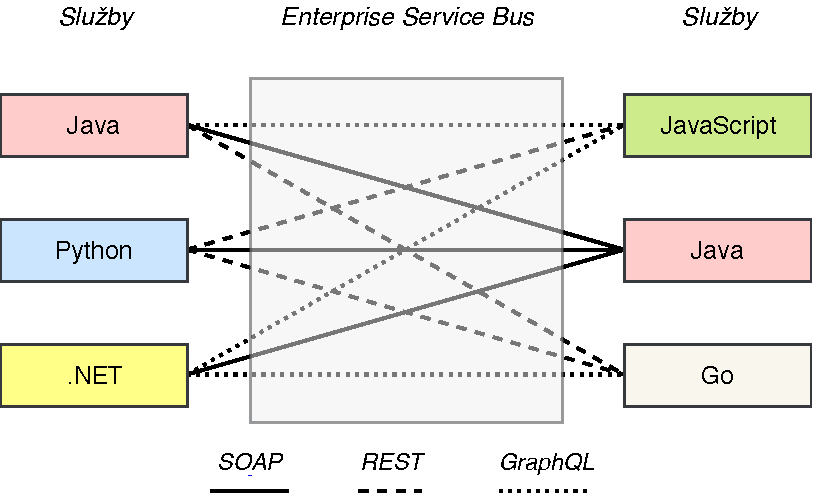
\includegraphics[keepaspectratio=true, width=0.8\linewidth]{figures/enterprise-service-bus.pdf}
    \caption{Komunikace služeb skrz Enterprise Service Bus}
    \label{fig:enterprise-service-bus}
\end{figure}

\goal{Ambiguita termínu SOA v historii}
Historicky byl termín SOA vykládán různými způsoby a vývojáři si
pod nám představovali několik rozdílných, nekompatibilních
konceptů~\cite{fowler2005serviceorientedambiguity}.
Zejména pak absence kvalitních definicí toho, co vlastně
služba je, vedla k vzájemnému nedorozumění, zmatení a postupném
zanevření nad touto architekturou.

\subsection{Microservices}

\goal{Microservices a budoucnost SOA}
Novým trendem posledních let jsou takzvané \textit{Microservices}.
Přináší několik zajmavých konceptů, které specializují a konkretizují
principy SOA. Microservices se tedy dají chápat jako podmnožina
SOA. Základní myšlenkou je vývoj informačního systému jako množiny
malých oddělených služeb, které jsou spouštěny v samostatných procesech
a komunikují spolu pomocí jednoduchých protokolů~\cite{lewis2014microservices}.

\goal{Stavba služeb kolem byznysových schopností}
Důležitou myšlenkou microservices je organizace služeb kolem
byznysových schopností systému. Namísto horizontálního dělení monolitu
podle jeho vrstev\footnote{
Zde předpokládáme klasickou třívrstvou architekturu~\cite{fowler2002patterns},
která rozděluje systém do vrstev s odlišnou zodpovědností,
přičemž sousední vrstvy spolu komunikují pomocí jasně definovaných společných rozhraní.
Těmito vrstvami jsou: \textit{datová vrstva}, \textit{aplikační vrstva} a \textit{prezentační vrstva}.
} diktuje rozdělit monolit vertikálně podle jeho byznysových schopností.
Na obrázku~\ref{fig:monolith-vs-microservices} je toto rozdělení demonstrováno.
Příkladem může být dělení e-commerce systému na jednu službu obsahující byznysovou
logiku pro registraci a správu uživatelů, druhou službu obsahující byznysovou logiku
pro práci s produkty a třetí službu obsahující byznysovou logiku pro práci
s objednávkami.

\begin{figure}
    \centering
    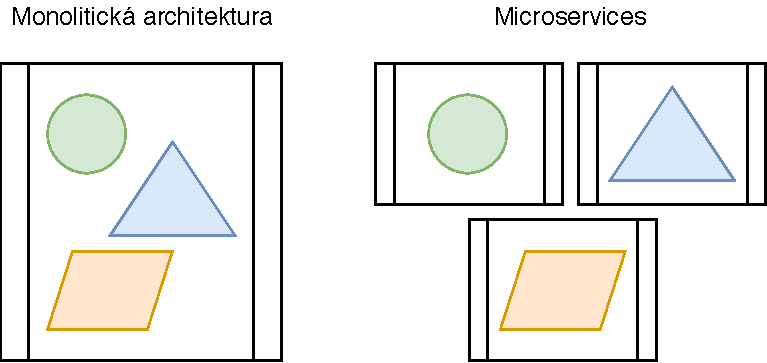
\includegraphics[keepaspectratio=true, width=0.8\linewidth]{figures/monolith-vs-microservices.pdf}
    \caption{Porovnání struktury monolitické architektury a microservices}
    \label{fig:monolith-vs-microservices}
\end{figure}

\goal{Myšlenka nahraditelnosti komponenty}
Koncept microservices přemýšlí o službě jako o samostatné komponentě,
kterou lze individuálně vyměnit či vylepšit, bez nutnosti zásahu do
ostatních služeb~\cite{lewis2014microservices}. Monolitická architektura
vyžaduje i při malé změně jedné části celý systém znovu zkompilovat, sestavit
a nasadit. Malé služby sloužící ideálně jedinému byznysovému účelu lze naopak
při změně byznysových požadavků snadno vyměnit samostatně bez zásahu do zbytku
systému. Tím se usnaďnuje cyklus nasazení a spuštění nové verze služby.

\goal{Myšlenka smart endpoints, dumb pipes}
Microservices také přinášejí koncept \uv{smart endpoint, dumb pipes},
který opouští koncept ESB ve prospěch přesunutí veškeré byznys logiky
na stranu služeb.

\goal{Škálovatelnost}
% TODO: napišmě

\begin{figure}
    \centering
    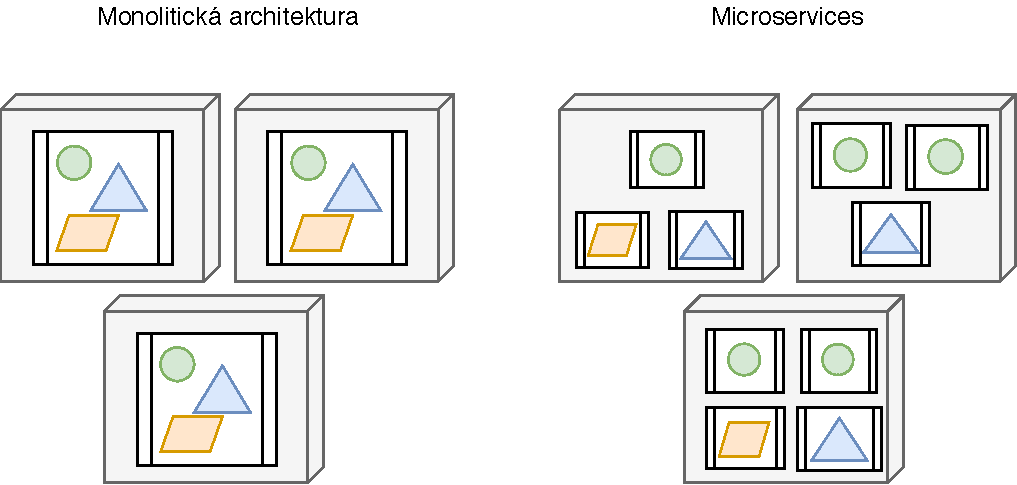
\includegraphics[keepaspectratio=true, width=0.8\linewidth]{figures/microservices-deployment.pdf}
    \caption{Porovnání nasazení monolitické architektury a microservices}
    \label{fig:microservices-deployment}
\end{figure}

~\cite{perrey2003service}
~\cite{cerny2017disambiguation}
~\cite{sprott2004understanding}

\subsection{Service discovery}

\goal{Service discovery}

\goal{Definice služby}
\paragraph{Služba} je ucelenou systémovou komponentou,
kterou lze nasadit a spustit jako samostatný proces, a
komunikuje s ostatními službami pomocí zpráv.

\section{Problémy}

\goal{Problémy microservices}
Jelikož jedním z cílů microservices je co nejvíce izolovat
jednotlivé služby, mají tendenci duplikovat znalosti, které
zasahují do více služeb najednou~\cite{cerny2017disambiguation}.
Zároveň tím ztrácíme

\section{Identifikace požadavků na implementaci frameworku}

\begin{itemize}
    \item{Definice byznys kontextů pomocí doménově specifického jazyka srozumitelného pro doménové experty}
    \item{Zápis preconditions a post-conditions pravidla jednotlivých byznys kontextů}
    \item{Automatická distribuce kontextů, vyhodnocování jejich preconditions a aplikace post-conditions}
    \item{Možnost jednoho kontextu rozšiřovat jiné kontexty}
    \item{Možnost centrálně spravovat byznysové kontexty, včetně úpravy stávajících a vytváření nových kontextů}
\end{itemize}

\section{Shrnutí}

V této kapitole jsme nastínili problematiku vysoké komplexity moderních informačních systémů
a z toho vyplívající požadavky na jejich architekturu. Analyzovali jsme koncept byznysových
pravidel a byznysových kontextů. Dále jsme zkomali architekturu orientovanou na služby, její
výhody a nevýhody, její moderní evoluci v podobě Microservices a identifikovali jsme problémy
v souvislosti s byznysovými pravidly, která zasahují do jednotlivých služeb. Nakonec jsme
vyjmenovali požadavky, které by měl splňovat framework, který bude výstupem této práce.
